\chapter{The Impossibility Theorem: Why the Wall Is
Necessary}

Every experimental chapter met the same wall: on average-case matching
the advice-free baseline is near-optimal, predictions buy robustness
insurance rather than performance, and --- for the test-and-fallback
algorithms --- no acceptance threshold both captures the tiny upside and
stays safe (Chapter 6). This chapter argues the wall is not an accident
of a particular threshold, graph, or algorithm, but a \emph{theorem}. To
keep the exposition focused we give the intuition and the architecture
of the proof here, and defer the full formal development to Appendix B.

\section{The claim}

Informally:

\begin{quote}
On strong-baseline instances, no test-and-fallback algorithm whose test
inspects only a \textbf{sublinear} prefix of the arrivals can be both
consistent and robust.
\end{quote}

A \emph{test-and-fallback} algorithm (Chapter 3) observes the first
\(k\) arrivals, decides --- by \emph{any} rule --- whether to follow the
advice or fall back to Ranking, and commits. The claim is that when the
budget \(k\) is sublinear (\(k=o(n)\)) and the baseline is strong, the
achievable (consistency, robustness) region collapses to the single
point ``just play the baseline'': one can be safe, or capture the
upside, but not both.

\textbf{Figure 9.1} is the empirical face of this. As the baseline
weakens (moving right to left), the \emph{potential} upside --- how much
perfect advice beats the baseline --- grows; but the upside a sublinear
test can \emph{safely capture} stays pinned near zero. The gap between
the two curves is the impossibility.

\begin{figure}
\centering
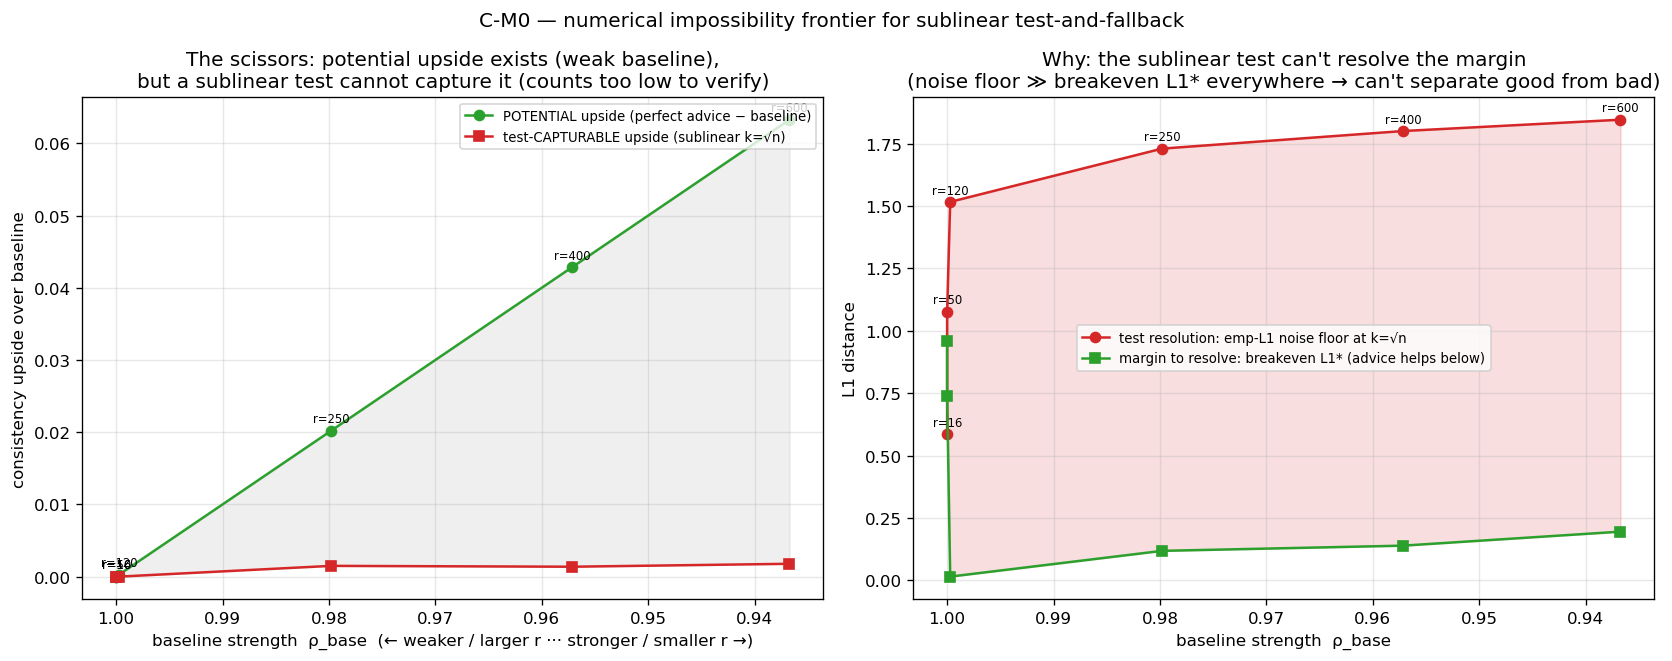
\includegraphics[width=1\linewidth,height=\textheight,keepaspectratio,alt={The impossibility, numerically (the ``scissors''). Left: the potential upside grows as the baseline weakens, but the upside a sublinear test can safely capture stays near zero. Right: the test's empirical-\textbackslash ell\_1 resolution sits far above the break-even margin wherever an upside exists.}]{../../results/impossibility_frontier.png}
\caption{The impossibility, numerically (the ``scissors''). Left: the
\emph{potential} upside grows as the baseline weakens, but the upside a
sublinear test can \emph{safely capture} stays near zero. Right: the
test's empirical-\(\ell_1\) resolution sits far above the break-even
margin wherever an upside exists.}
\end{figure}

\section{The intuition: testability and baseline strength are the same
knob}

The heart of the argument is a coupling that is easy to state and, once
seen, hard to un-see. To decide safely whether to trust the advice, the
algorithm must, from its short prefix, tell \emph{good} advice (close
enough to the truth to help) from \emph{bad} advice (far enough to
hurt). This is a statistical test on the distribution of request types.
Such a test is only feasible when there are \textbf{few types, each
arriving many times} --- otherwise the prefix is too sparse to estimate
anything. But few high-count types is \emph{exactly} the regime in which
the matching is near-perfect and the advice-free baseline is already
near-optimal, so there is nothing worth testing for. Where the baseline
is weak enough that advice could genuinely help, the types are many and
each is seen only a handful of times, and no sublinear prefix can run
the test.

In one sentence: \textbf{the structure that makes the test feasible is
the structure that makes the baseline near-optimal --- so wherever you
can test the advice, you do not need it.} The rest of the chapter turns
this intuition into a proof.

\section{The architecture of the
proof}

The proof rests on three pillars; we state each in words and give its
one key formula, leaving the formal details to Appendix B.

\textbf{Pillar 1 --- a trade-off inequality (rigorous).} If two
instances that require \emph{opposite} decisions (follow vs fall back)
look statistically the same over the prefix --- that is, their prefix
distributions have small total-variation distance \(\gamma_k\) --- then
no rule on the prefix can serve both. Formally, writing \(\eta_c\) for
the fraction of the upside an algorithm forgoes and \(\eta_r\) for its
robustness loss, one shows \[(1-\eta_c)\;\le\;\eta_r+\gamma_k+o(1).\]
When the prefix is uninformative (\(\gamma_k\to0\)) the algorithm cannot
be both consistent (\(\eta_c\to0\)) and robust (\(\eta_r\to0\)). This
lemma is short and self-contained; it is the two-sided core of the
result.

\textbf{Pillar 2 --- a reduction to distribution testing (any rule).}
The prefix is \emph{literally} a set of i.i.d. samples from the type
distribution. We build a family in which following the advice helps
exactly when the advice is \(\ell_1\)-close to the truth and hurts
exactly when it is \(\ell_1\)-far; on it, a consistent-and-robust
algorithm would in effect \emph{distinguish close from far from the
samples} --- a \textbf{tolerant} distribution-testing problem. Because
the algorithm's decision is an arbitrary function of the samples, the
lower bound below rules out \emph{every} rule, not just the
empirical-distance threshold used in practice --- which is what
distinguishes our result from the constructive baseline-coupling already
present in Choo et al.'s algorithm.

\textbf{Pillar 3 --- tolerant testing is nearly as hard as learning the
distribution.} The final ingredient is a known and, at first, surprising
fact from distribution testing. \emph{Verifying} that a distribution
equals a known one needs only \(\Theta(\sqrt r)\) samples --- sublinear
in the number of types \(r\). But \emph{tolerant} testing ---
distinguishing ``somewhat close'' from ``somewhat far,'' which is what
safe advice-use requires --- needs \(\tilde\Theta(r/\log r)\) samples,
nearly \emph{linear} in \(r\)
\autocite{canonne2022tolerance,valiant2011unseen}. Our construction has
\(r=\Theta(n)\) types, so the test needs \(\tilde\Theta(n/\log n)\)
samples --- more than any sublinear prefix provides. The good-advice
side is genuinely a \emph{ball} around the truth (not a single point),
which is what places the problem in the hard tolerant regime rather than
the easy \(\sqrt r\) one. A side benefit of the construction is that the
map from advice error to matching loss is an \emph{exact linear law}
(verified numerically), which pins the constants cleanly.

Chaining the three: on the family, any \((1-o(1))\)-consistent, robust,
sublinear-test algorithm would solve a tolerant test it provably cannot,
so no such algorithm exists.

\section{The theorem}

\begin{quote}
\textbf{Theorem (informal).} For every sublinear test budget
\(k=o(n/\log n)\) there is a known-i.i.d. matching family with
\(\Theta(n)\) types and a strong baseline on which no test-and-fallback
algorithm --- by any rule on its prefix --- is simultaneously
\((1-o(1))\)-consistent and robust. The achievable (robustness,
consistency) region collapses to the baseline point.
\end{quote}

Together with the easy strong-baseline side (few types \(\Rightarrow\)
near-optimal baseline \(\Rightarrow\) no upside to capture), this is
precisely the scissors of Figure 9.1, now with a proof: the upside lives
only where the tolerant test is infeasible.

\section{Scope, status, and honesty}

\textbf{Scope.} The strong form is stated for the regime with
\(\Theta(n)\) types --- which is the only regime with an upside to
contest, and hence the natural one; a version that also bites at
constant \(r\) is left open. The reduction inherits the
empirical-\(\ell_1\) modeling of the test used by the algorithms it
bounds (Chapter 3).

\textbf{Relation to prior work.} Choo et al.~and BEM give algorithms
(upper bounds) and no lower bound in this model; Choo et al.'s threshold
already couples to the baseline ratio, but \emph{constructively}. Our
contribution is the two-sided, \emph{rule-independent} impossibility and
the identification of testability with baseline strength; the reduction
from distribution-testing sample complexity to the value of advice in an
online algorithm is, to our knowledge, new.

\textbf{Status (stated plainly).} The trade-off inequality (Pillar 1) is
proved; the construction's constants and the linear conversion law are
derived and numerically verified; the tolerant-testing barrier (Pillar
3) is a cited, exact result on the theorem-preserving side of the
tolerant/non-tolerant divide. One routine step of the construction ---
exhibiting the two indistinguishable witness distributions guaranteed by
the testing lower bound --- and a final review remain before the full
proof is complete. The thesis presents the theorem with this status
stated, as befits in-progress theoretical work; the empirical scissors
of Figure 9.1 is independent evidence that the statement is true.
